%\newpage
\section{Simulation}

\subsection{Erläuterung zu der Simulation}
Gemäss Simulation sollte die Antenne einen Reflexionsfaktor von knapp
\SI{-25}{\dB} aufweisen bei einer Frequenz von \SI{2.4}{\giga\hertz}.
Bei \SI{5}{\giga\hertz} sollte dieser bei \SI{-17}{\dB} liegen. Abbildung
\ref{fig:reflexionsfaktor} auf Seite \pageref{fig:reflexionsfaktor}.

Die reale Impedanz liegt gemäss Simulation bei \SI{2.4}{\giga\hertz} bei
\SI{43}{\ohm}, der Imaginäranteil bei \SI{10}{\ohm} kapazitiv. Bei
\SI{5}{\giga\hertz} liegt der Realanteil bei \SI{40}{\ohm} und der
Imaginäranteil bei \SI{6}{\ohm}. Abbildung \ref{fig:impedanz} auf
Seite \pageref{fig:impedanz}. Auf Seite \pageref{fig:electricfield}
sind in Abbildungen \ref{fig:electricfield_2_4} und \ref{fig:electricfield_5_0}
das elektrische Feld für \SI{2.4}{\giga\hertz} und \SI{5}{\giga\hertz}
abgebildet. Die Simulation zeigt schön, wie sich das elektrische Feld
je nach Frequenz unterschiedlich ausprägt. Auch die Simulation für die
Oberflächenstromdichte zeigt ein ausgeprägtes Verhalten, je nach
angelegter Frequenz. Abgebildet auf Seite \pageref{fig:currentdensity}
in Abbildungen \ref{fig:currentdensity_2_4} und \ref{fig:currentdensity_5_0}.


\clearpage
\subsubsection{Reflexionsfaktor $S_{11}$}
\begin{figure}[h!]
	\centering
	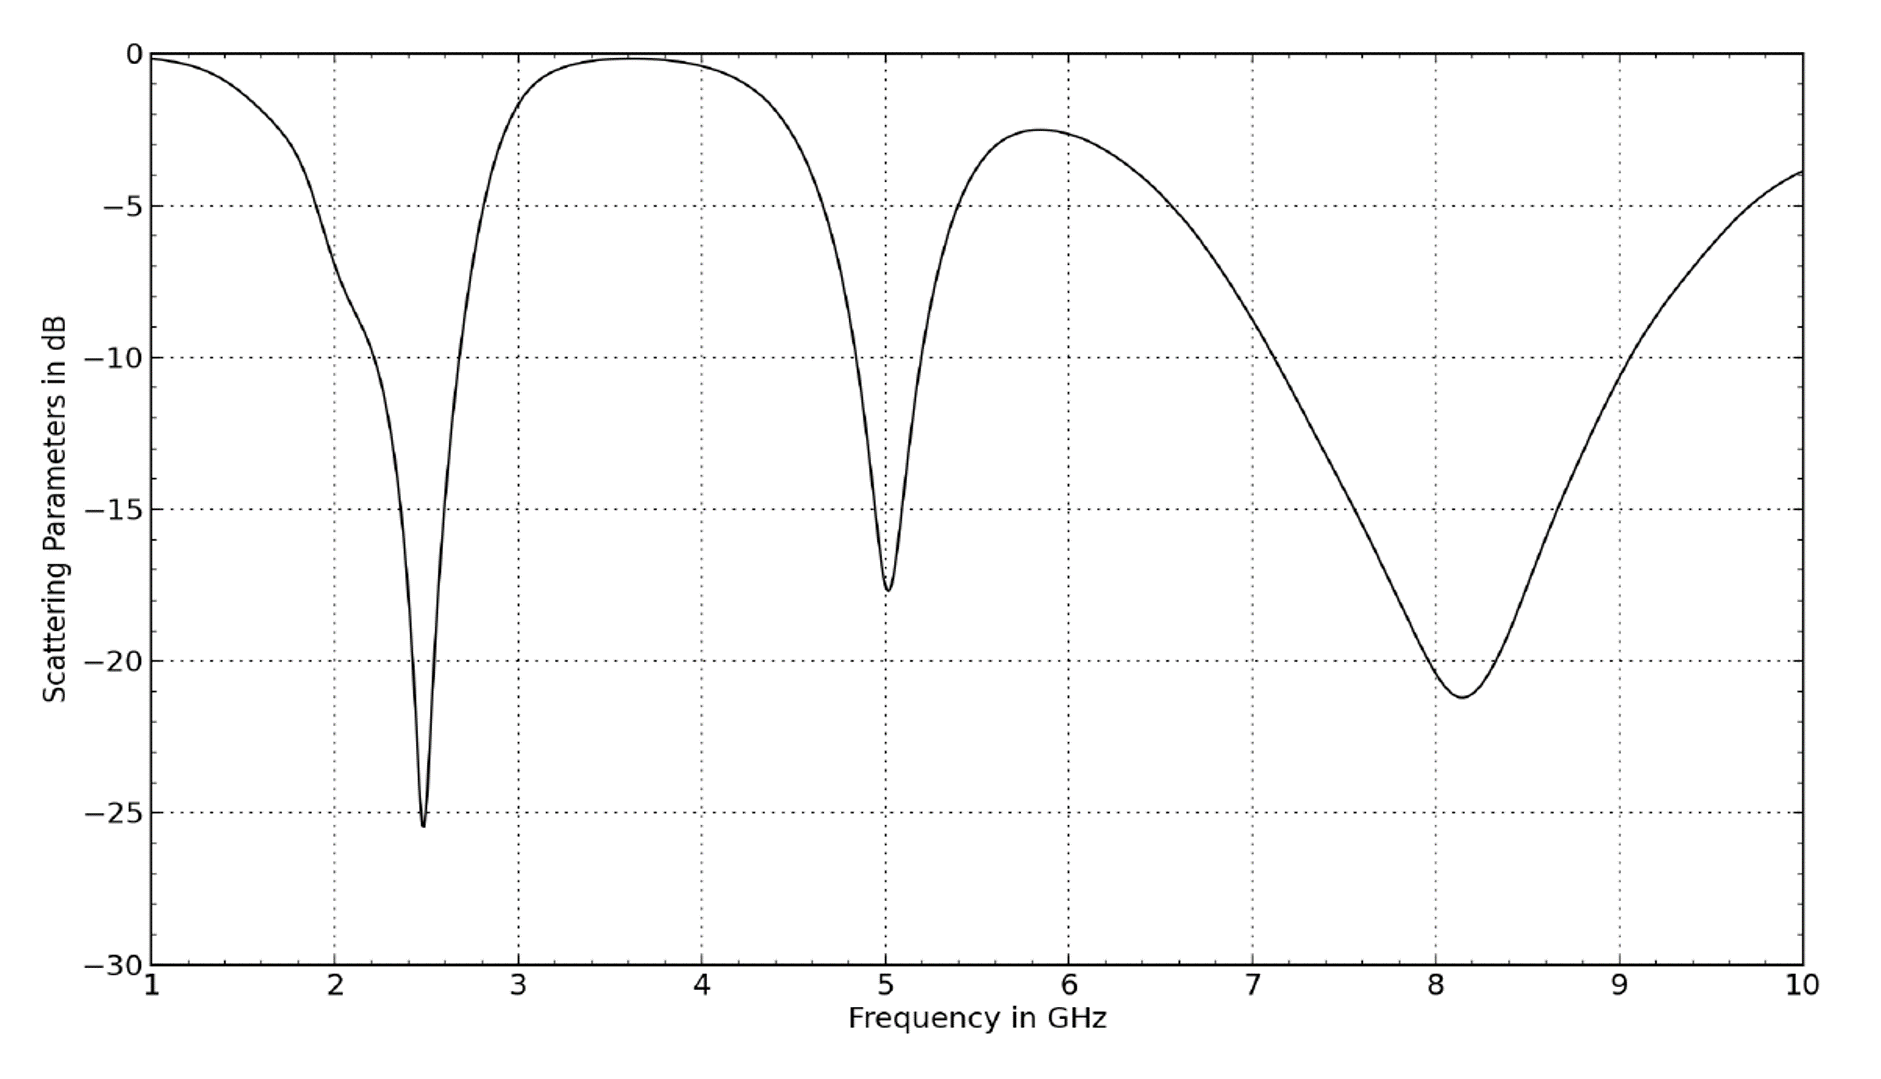
\includegraphics[width=0.7\textwidth]{../fig/plt/crazy_stuff_l4_pcb_v2c_laptop_1a_105_S11_2.png}
	\caption{Reflexionsfaktor $S_{11}$}
	\label{fig:reflexionsfaktor}
\end{figure}

%\clearpage
\subsubsection{Impedanz}
\begin{figure}[h!]
	\centering
	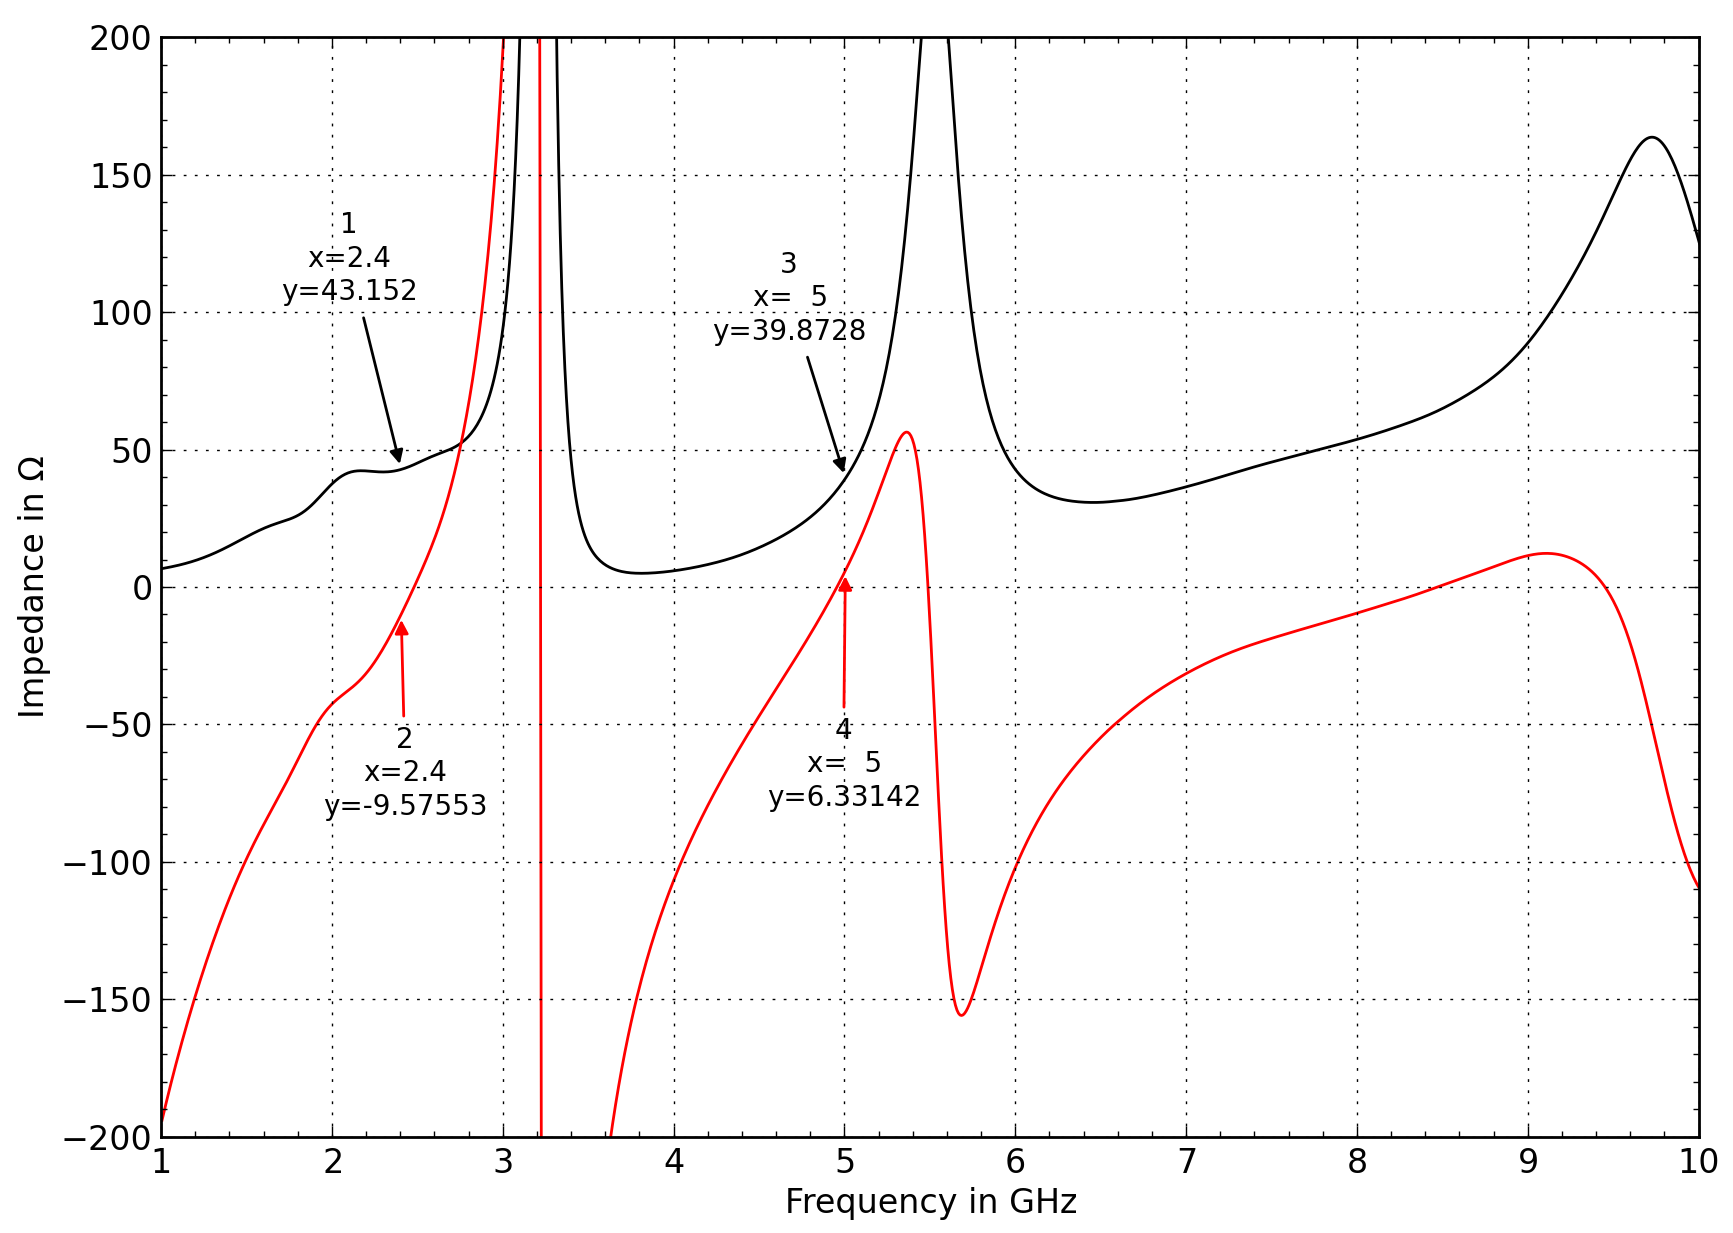
\includegraphics[width=0.7\textwidth]{../fig/plt/crazy_stuff_l4_pcb_v2c_laptop_1a_105_Widerstand_1.png}
	\caption{Impedanz}
	\label{fig:impedanz}
\end{figure}

\newpage
\subsubsection{Elektrisches Feld}
\begin{figure}[h!]
	\begin{center}
		\begin{subfigure}[t]{0.49\textwidth}
			\begin{center}
				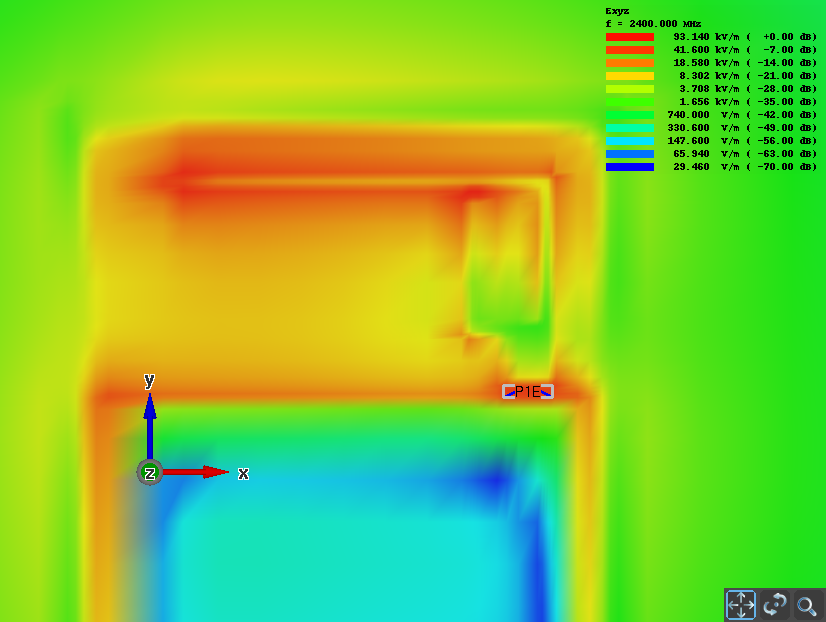
\includegraphics[width=0.94\textwidth]{../fig/plt/crazy_stuff_l4_pcb_v2c_laptop_1a_105_2ghz4_3d_electric_field_xy.png}
				\caption{bei 2.4 GHz}
				\label{fig:electricfield_2_4}
			\end{center}
		\end{subfigure}
		\begin{subfigure}[t]{0.49\textwidth}
			\begin{center}
				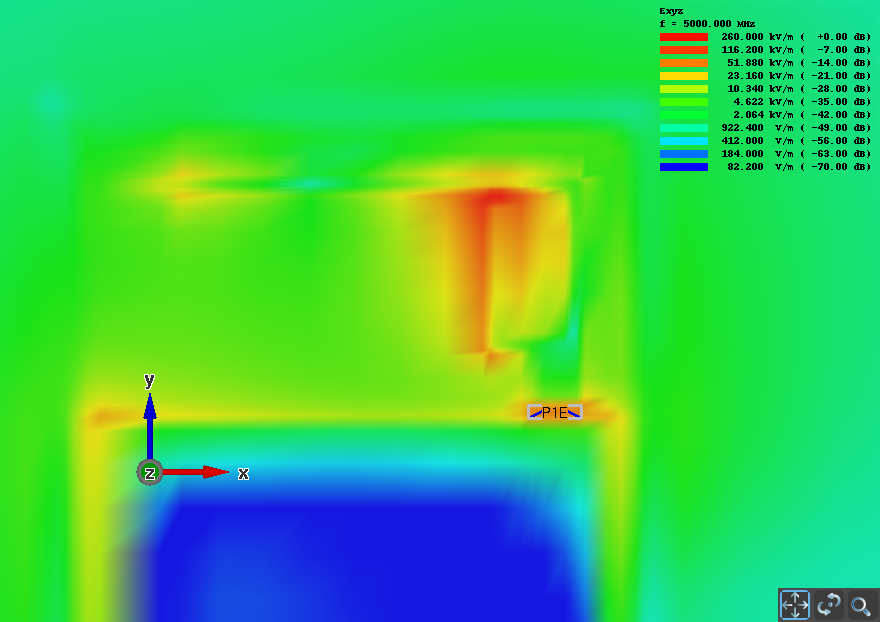
\includegraphics[width=1\textwidth]{../fig/plt/crazy_stuff_l4_pcb_v2c_laptop_1a_105_5ghz_3d_electric_field_xy.png}
				\caption{bei 5.0 GHz}
				\label{fig:electricfield_5_0}
			\end{center}
		\end{subfigure}
		\caption{Elektrisches Feld}
		\label{fig:electricfield}
	\end{center}
\end{figure}

\subsubsection{Oberflächenstromdichte}
\begin{figure}[h!]
	\begin{center}
		\begin{subfigure}[t]{0.49\textwidth}
			\begin{center}
				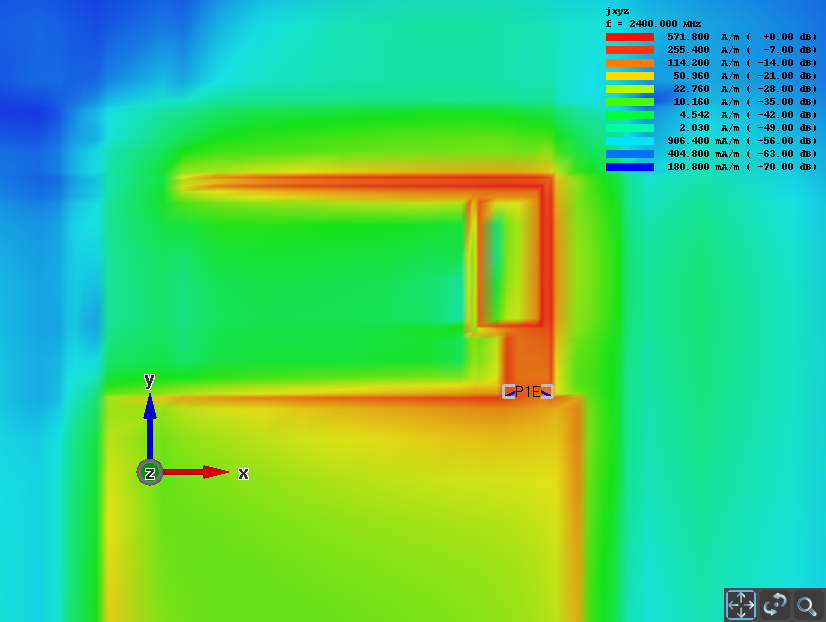
\includegraphics[width=0.94\textwidth]{../fig/plt/crazy_stuff_l4_pcb_v2c_laptop_1a_105_2ghz4_3d_surface_current_density_xy.png}
				\caption{bei 2.4 GHz}
				\label{fig:currentdensity_2_4}
			\end{center}
		\end{subfigure}
		\begin{subfigure}[t]{0.49\textwidth}
			\begin{center}
				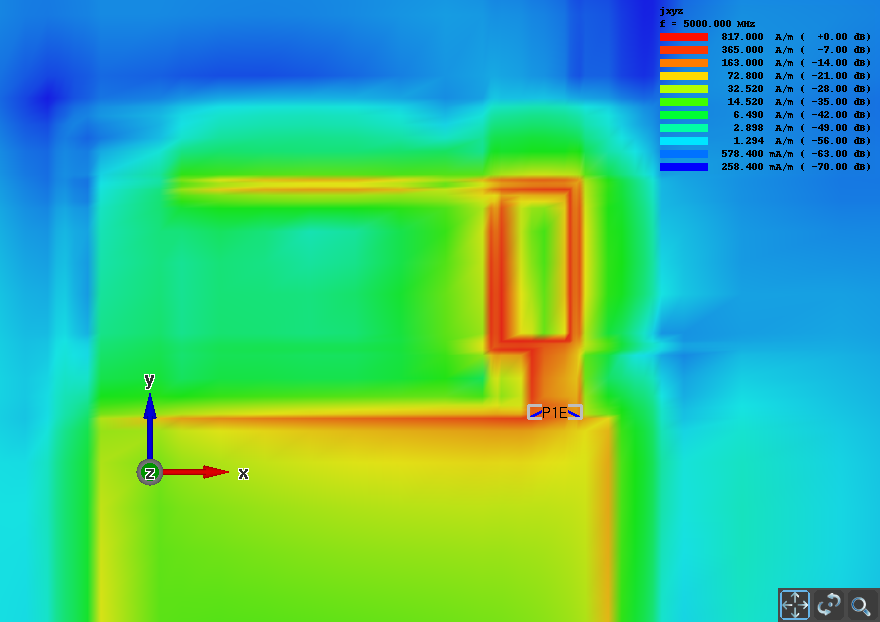
\includegraphics[width=1\textwidth]{../fig/plt/crazy_stuff_l4_pcb_v2c_laptop_1a_105_5ghz_3d_surface_current_density_xy.png}
				\caption{bei 5.0 GHz}
				\label{fig:currentdensity_5_0}
			\end{center}
		\end{subfigure}
		\caption{Oberflächenstromdichte}
		\label{fig:currentdensity}
	\end{center}
\end{figure}

\newpage
\subsubsection{Fernfeld bei 2.4 GHz}

\begin{figure}[h!]
	\centering
	\begin{subfigure}[b]{0.75\textwidth}
		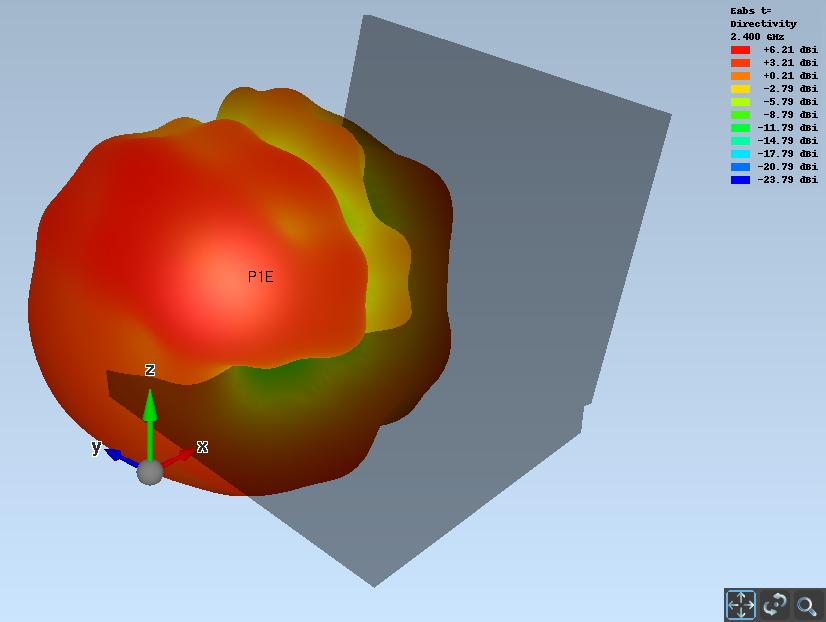
\includegraphics[width=1\textwidth]{../fig/plt/crazy_stuff_l4_pcb_v2c_laptop_1a_105_2ghz4_3d_farfield_eabs_xyz.png}
		\caption{$\vec{E}_{\mathrm{abs}}$}
	\end{subfigure}
	
	\vspace{3mm}
	
	\begin{subfigure}[b]{0.48\textwidth}
		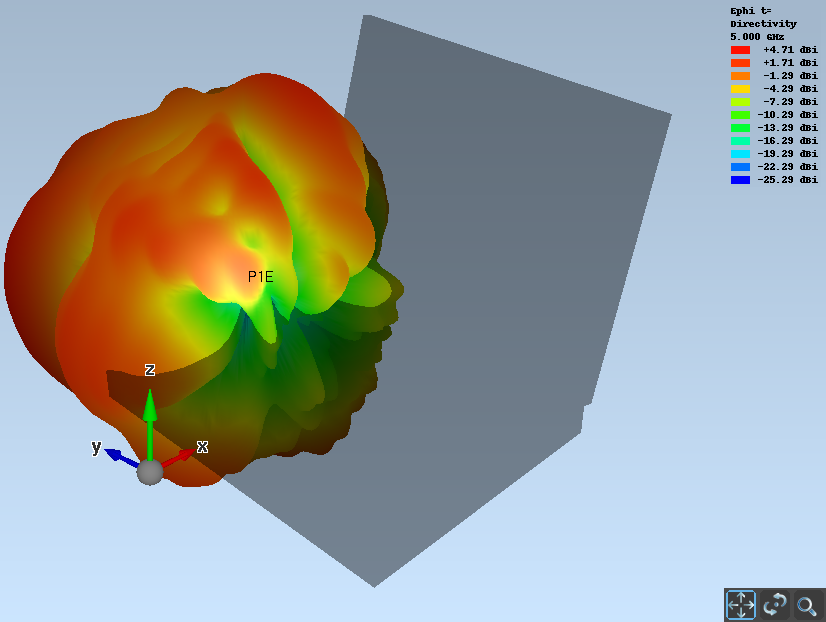
\includegraphics[width=1\textwidth]{../fig/plt/crazy_stuff_l4_pcb_v2c_laptop_1a_105_2ghz4_3d_farfield_ephi_xyz.png}
		\caption{$\vec{E}_{\varphi}$}
	\end{subfigure}
	\begin{subfigure}[b]{0.48\textwidth}
		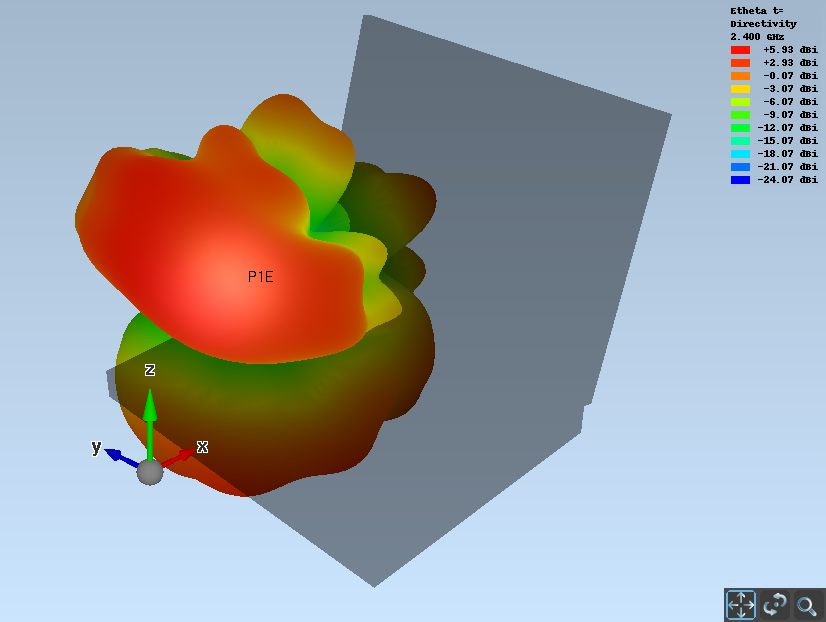
\includegraphics[width=1\textwidth]{../fig/plt/crazy_stuff_l4_pcb_v2c_laptop_1a_105_2ghz4_3d_farfield_etheta_xyz.png}
		\caption{$\vec{E}_{\Theta}$}
	\end{subfigure}
	\caption{$\vec{E}$ Fernfeldanalyse (3D) bei 2.4 GHz}
\end{figure}

In die Simulation wurde ein Laptopmodell miteinbezogen, in welchem der
USB-Dongle eingesteckt war. Der Bildschirm wurde mit einem Öffnungswinkel
von \SI{105}{\degree} simuliert.

\clearpage
\subsubsection{Fernfeld bei 5 GHz}
\begin{figure}[h!]
	\centering
	\begin{subfigure}[b]{0.75\textwidth}
		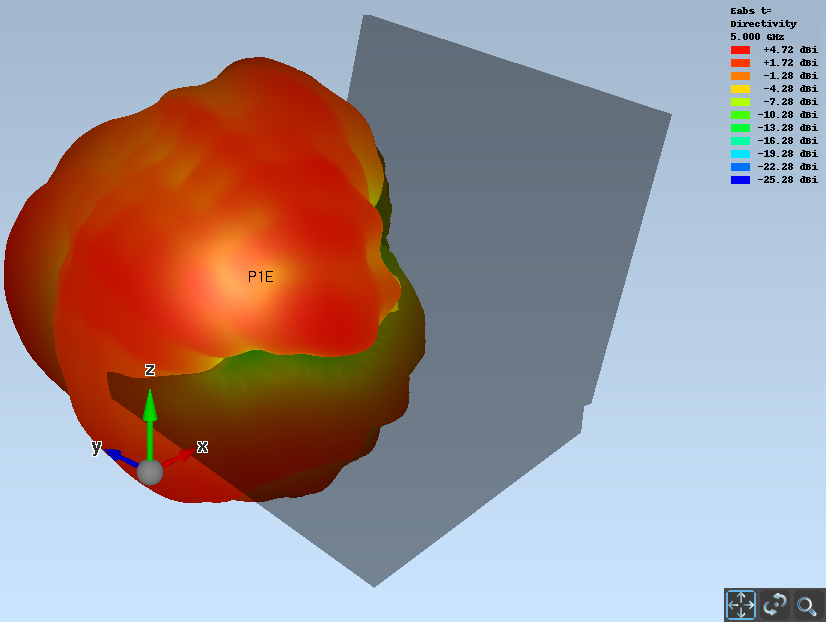
\includegraphics[width=1\textwidth]{../fig/plt/crazy_stuff_l4_pcb_v2c_laptop_1a_105_5ghz_3d_farfield_eabs_xyz.png}
		\caption{$\vec{E}_{\mathrm{abs}}$}
	\end{subfigure}

	\begin{subfigure}[b]{0.48\textwidth}
		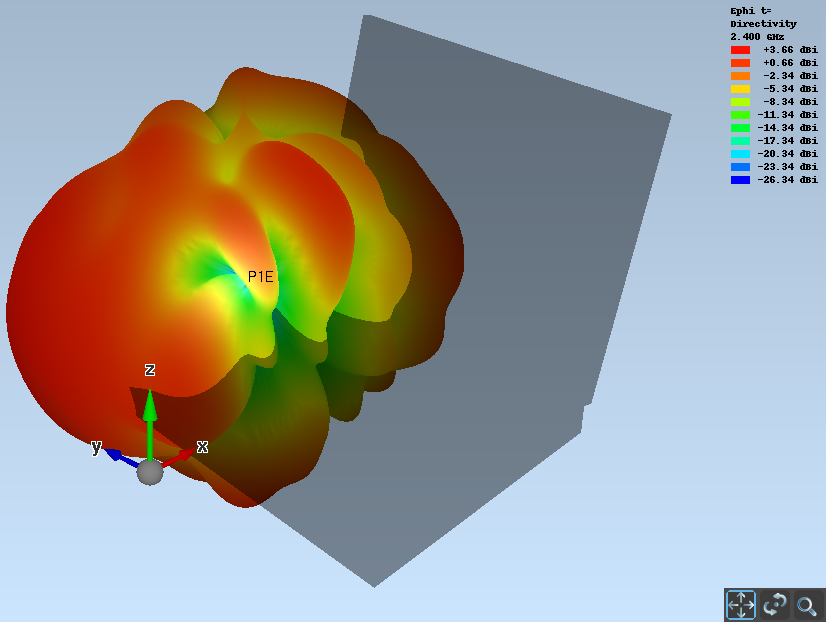
\includegraphics[width=1\textwidth]{../fig/plt/crazy_stuff_l4_pcb_v2c_laptop_1a_105_5ghz_3d_farfield_ephi_xyz.png}
		\caption{$\vec{E}_{\varphi}$}
	\end{subfigure}
	\begin{subfigure}[b]{0.48\textwidth}
		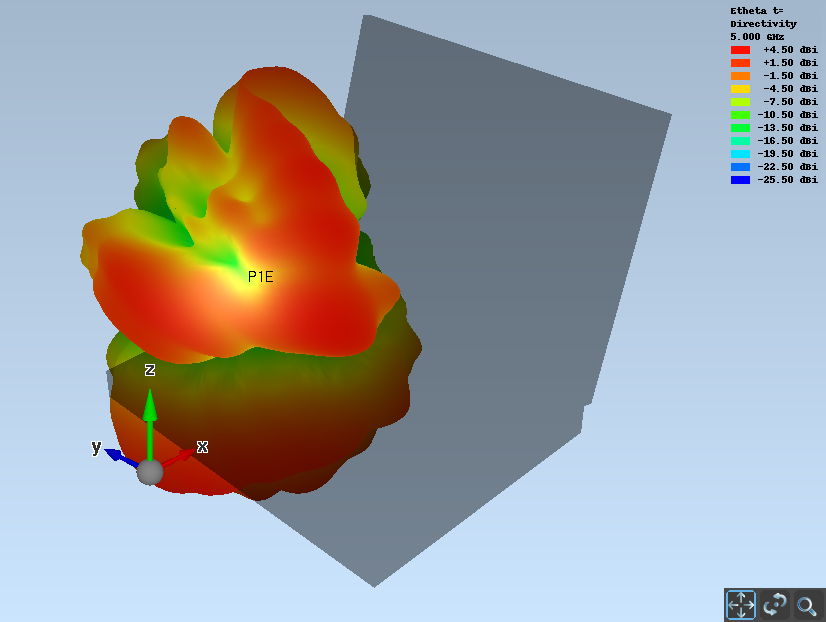
\includegraphics[width=1\textwidth]{../fig/plt/crazy_stuff_l4_pcb_v2c_laptop_1a_105_5ghz_3d_farfield_etheta_xyz.png}
		\caption{$\vec{E}_{\Theta}$}
	\end{subfigure}
	\caption{$\vec{E}$ Fernfeldanalyse (3D) bei 5.0 GHz}
\end{figure}



\clearpage
\subsubsection{Abstrahlung 1D}


\begin{figure}[h!]
	\centering
	\begin{subfigure}[b]{0.48\textwidth}
		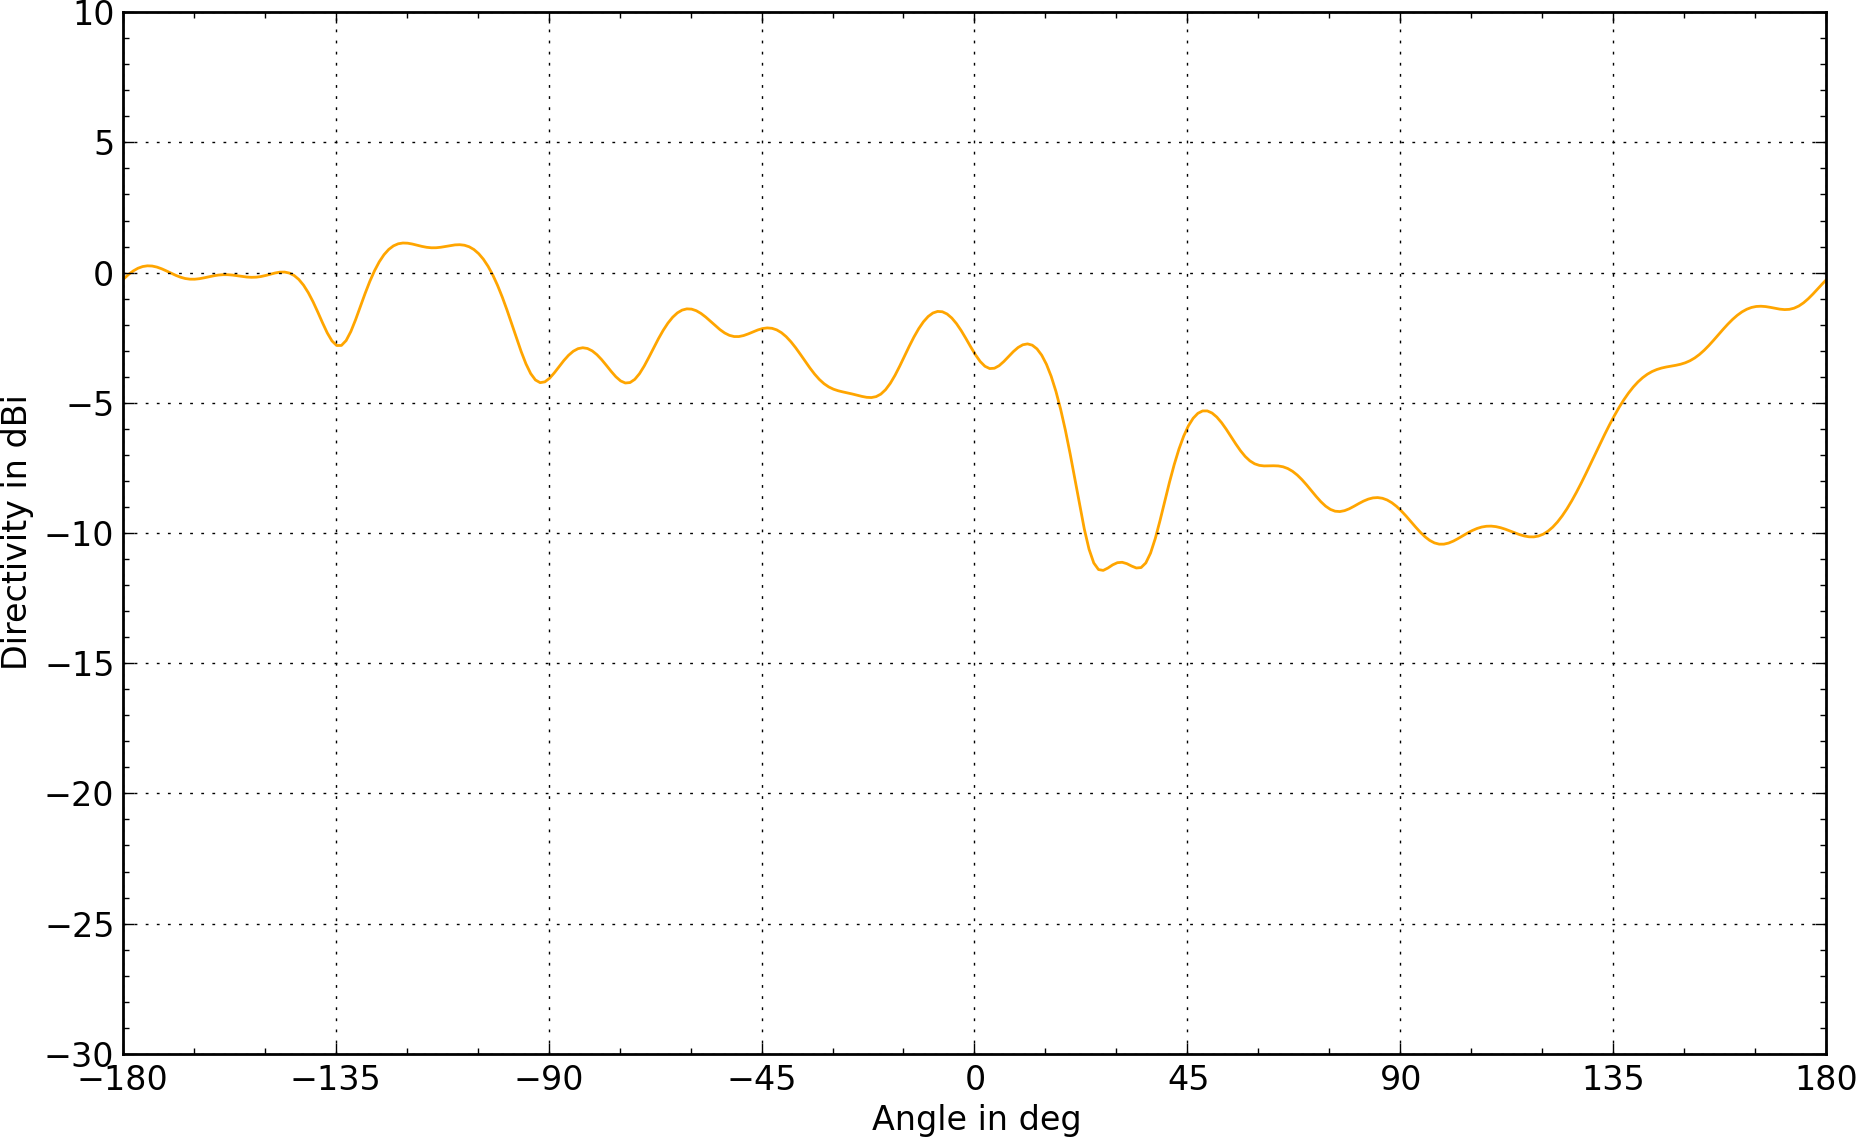
\includegraphics[width=1\textwidth]{../fig/plt/crazy_stuff_l4_pcb_v2c_laptop_1a_105_2ghz4_eabs_phi90-trim.png}
		\caption{$\vec{E_{tot}}$ mit $\varphi=\SI{90}{\degree}$ bei \SI{2.4}{\giga\hertz}}
	\end{subfigure}
	\begin{subfigure}[b]{0.48\textwidth}
		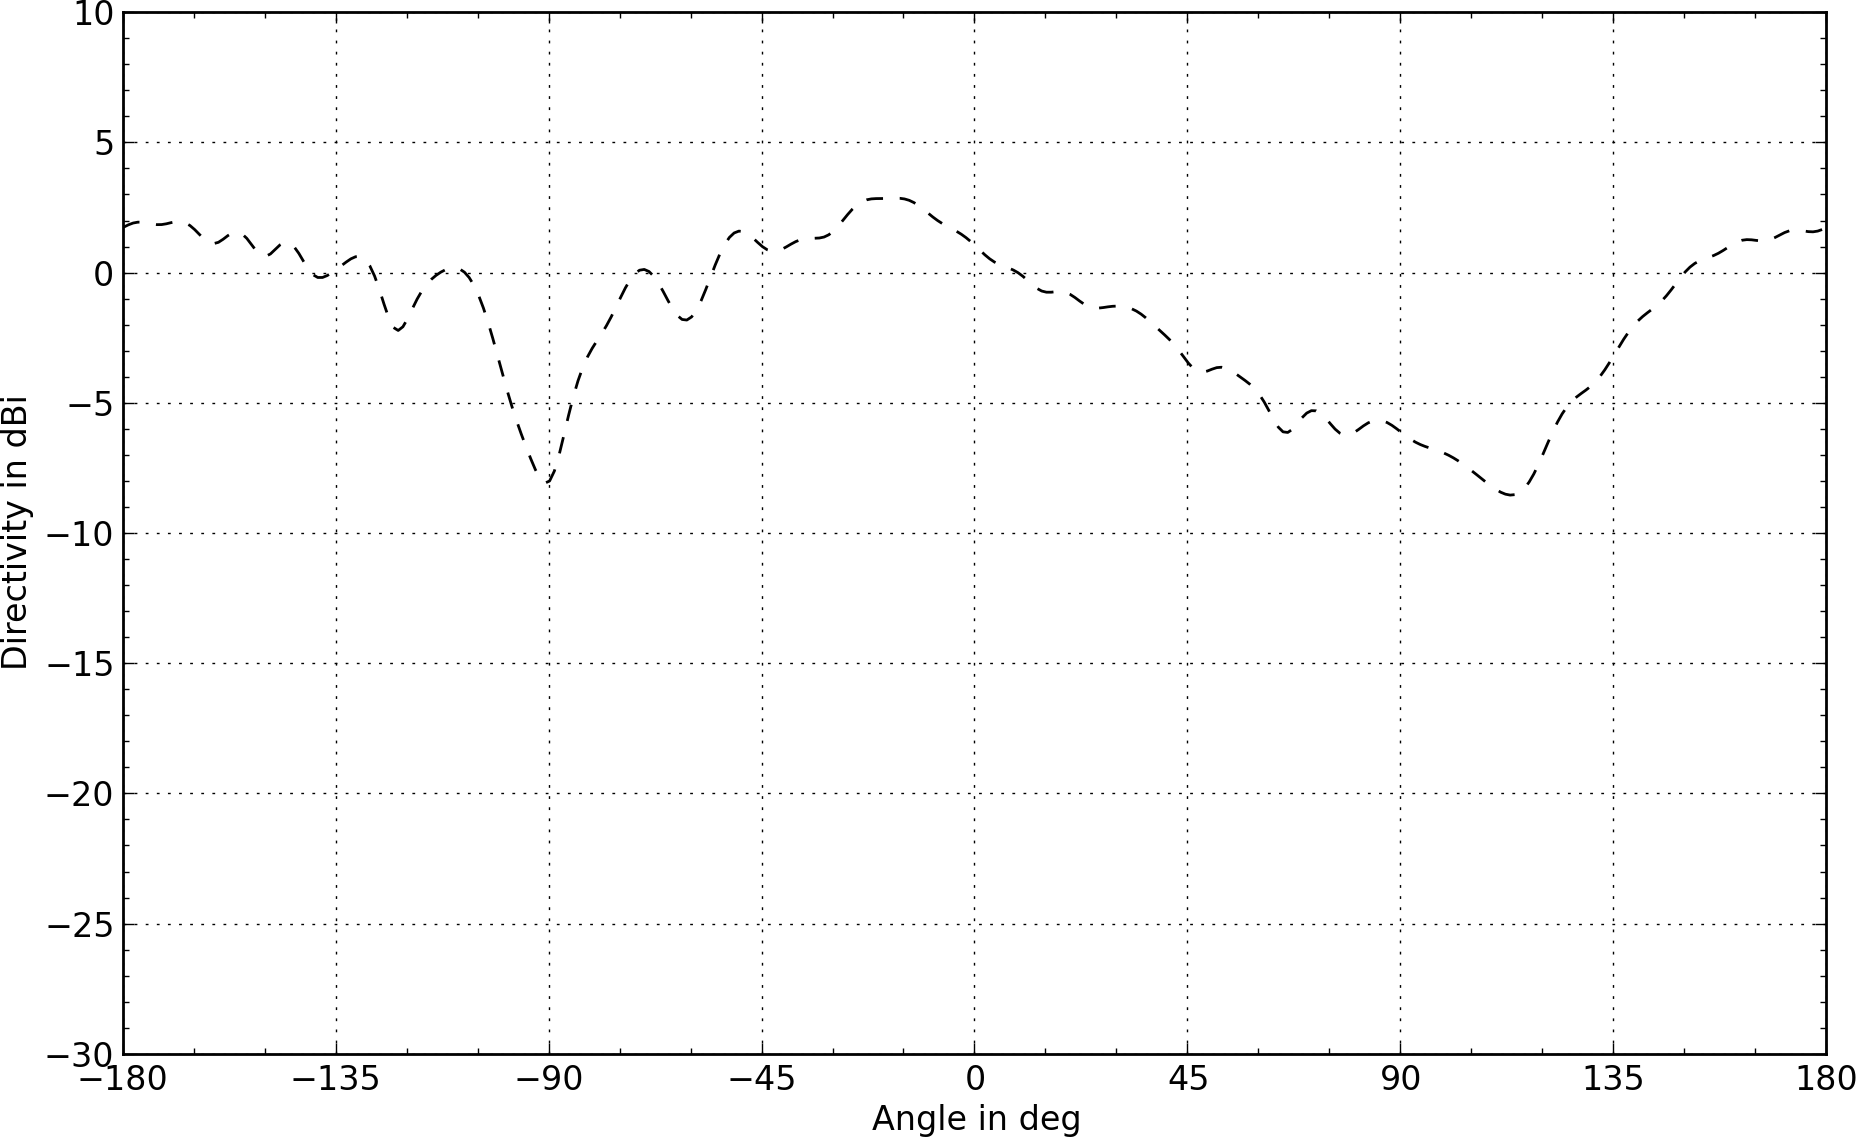
\includegraphics[width=1\textwidth]{../fig/plt/crazy_stuff_l4_pcb_v2c_laptop_1a_105_5ghz0_eabs_phi90-trim.png}
		\caption{$\vec{E_{tot}}$ mit $\varphi=\SI{90}{\degree}$ bei \SI{5.0}{\giga\hertz}}
	\end{subfigure}

	\begin{subfigure}[b]{0.48\textwidth}
		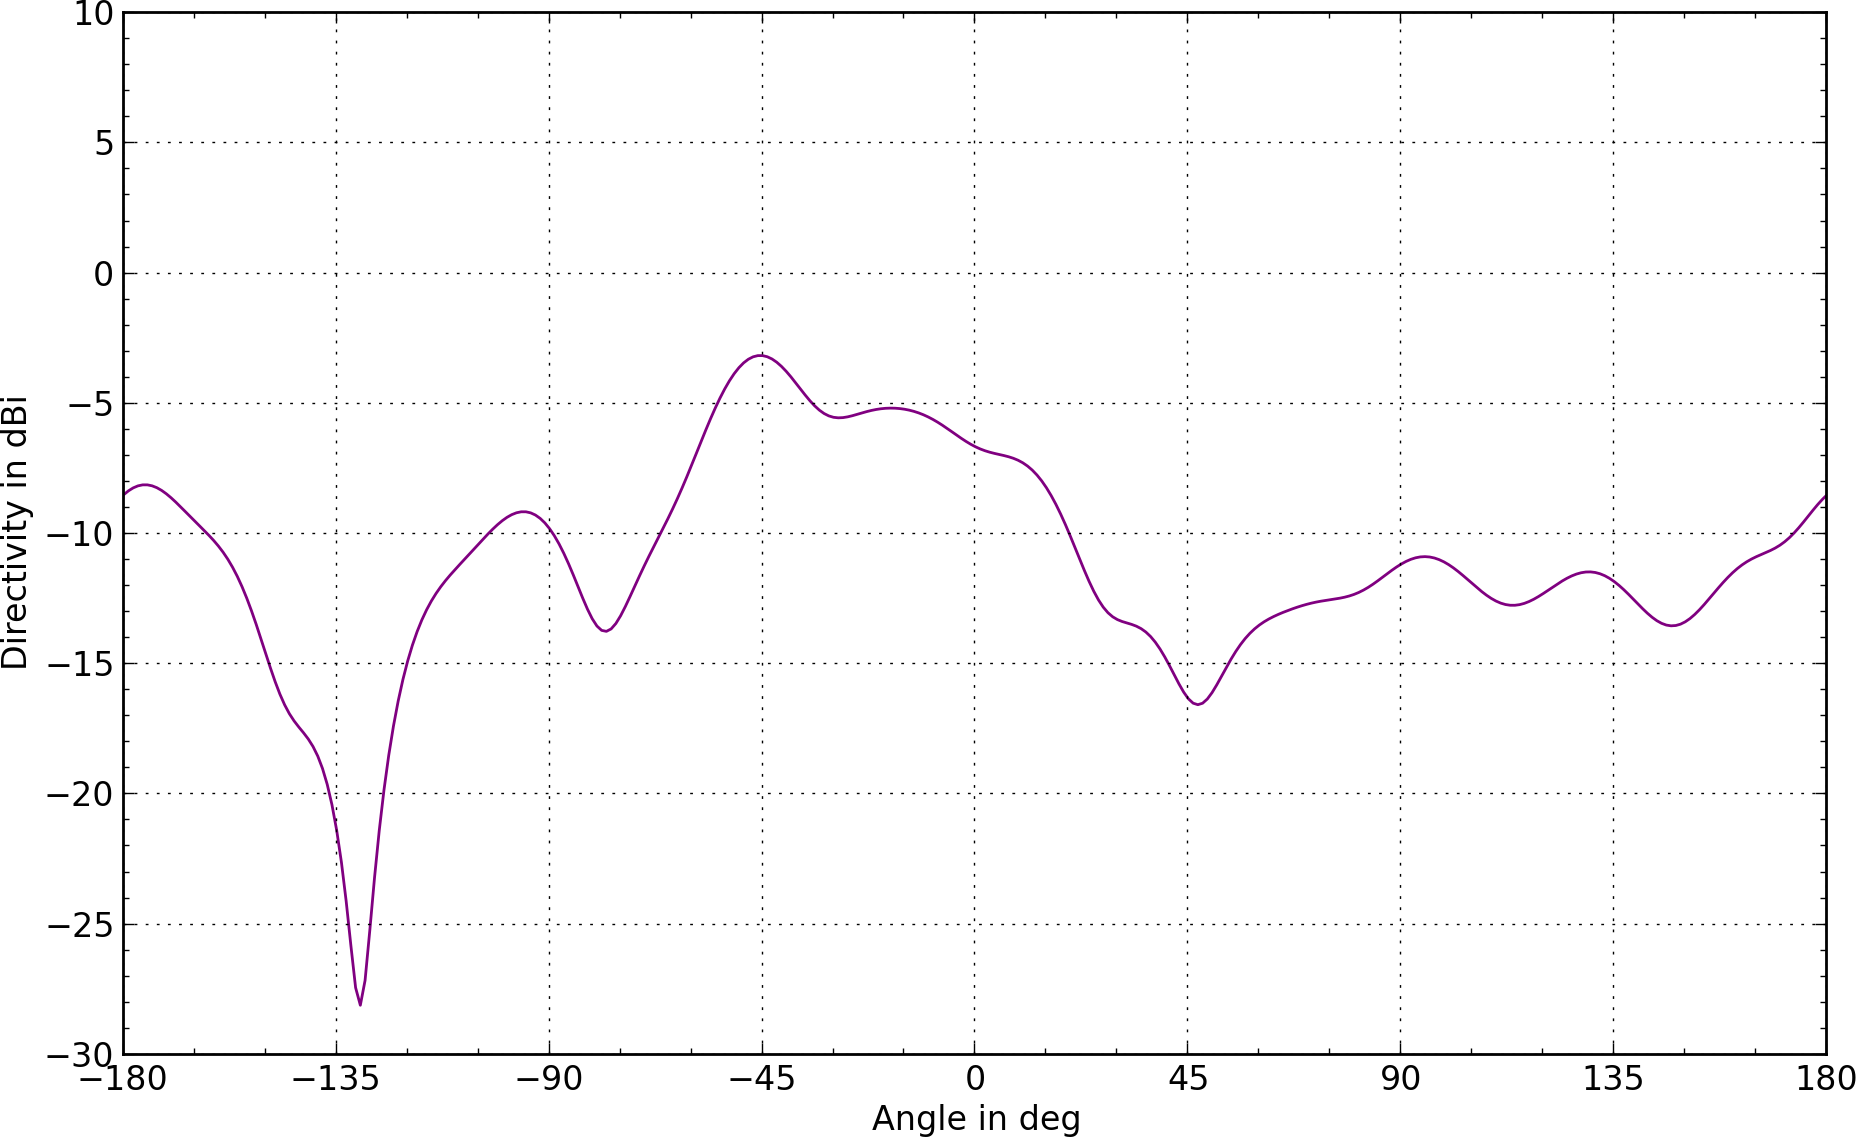
\includegraphics[width=1\textwidth]{../fig/plt/crazy_stuff_l4_pcb_v2c_laptop_1a_105_2ghz4_ephi_phi90-trim.png}
		\caption{$\vec{E_{\varphi}}$ mit $\varphi=\SI{90}{\degree}$ bei \SI{2.4}{\giga\hertz}}
	\end{subfigure}
	\begin{subfigure}[b]{0.48\textwidth}
		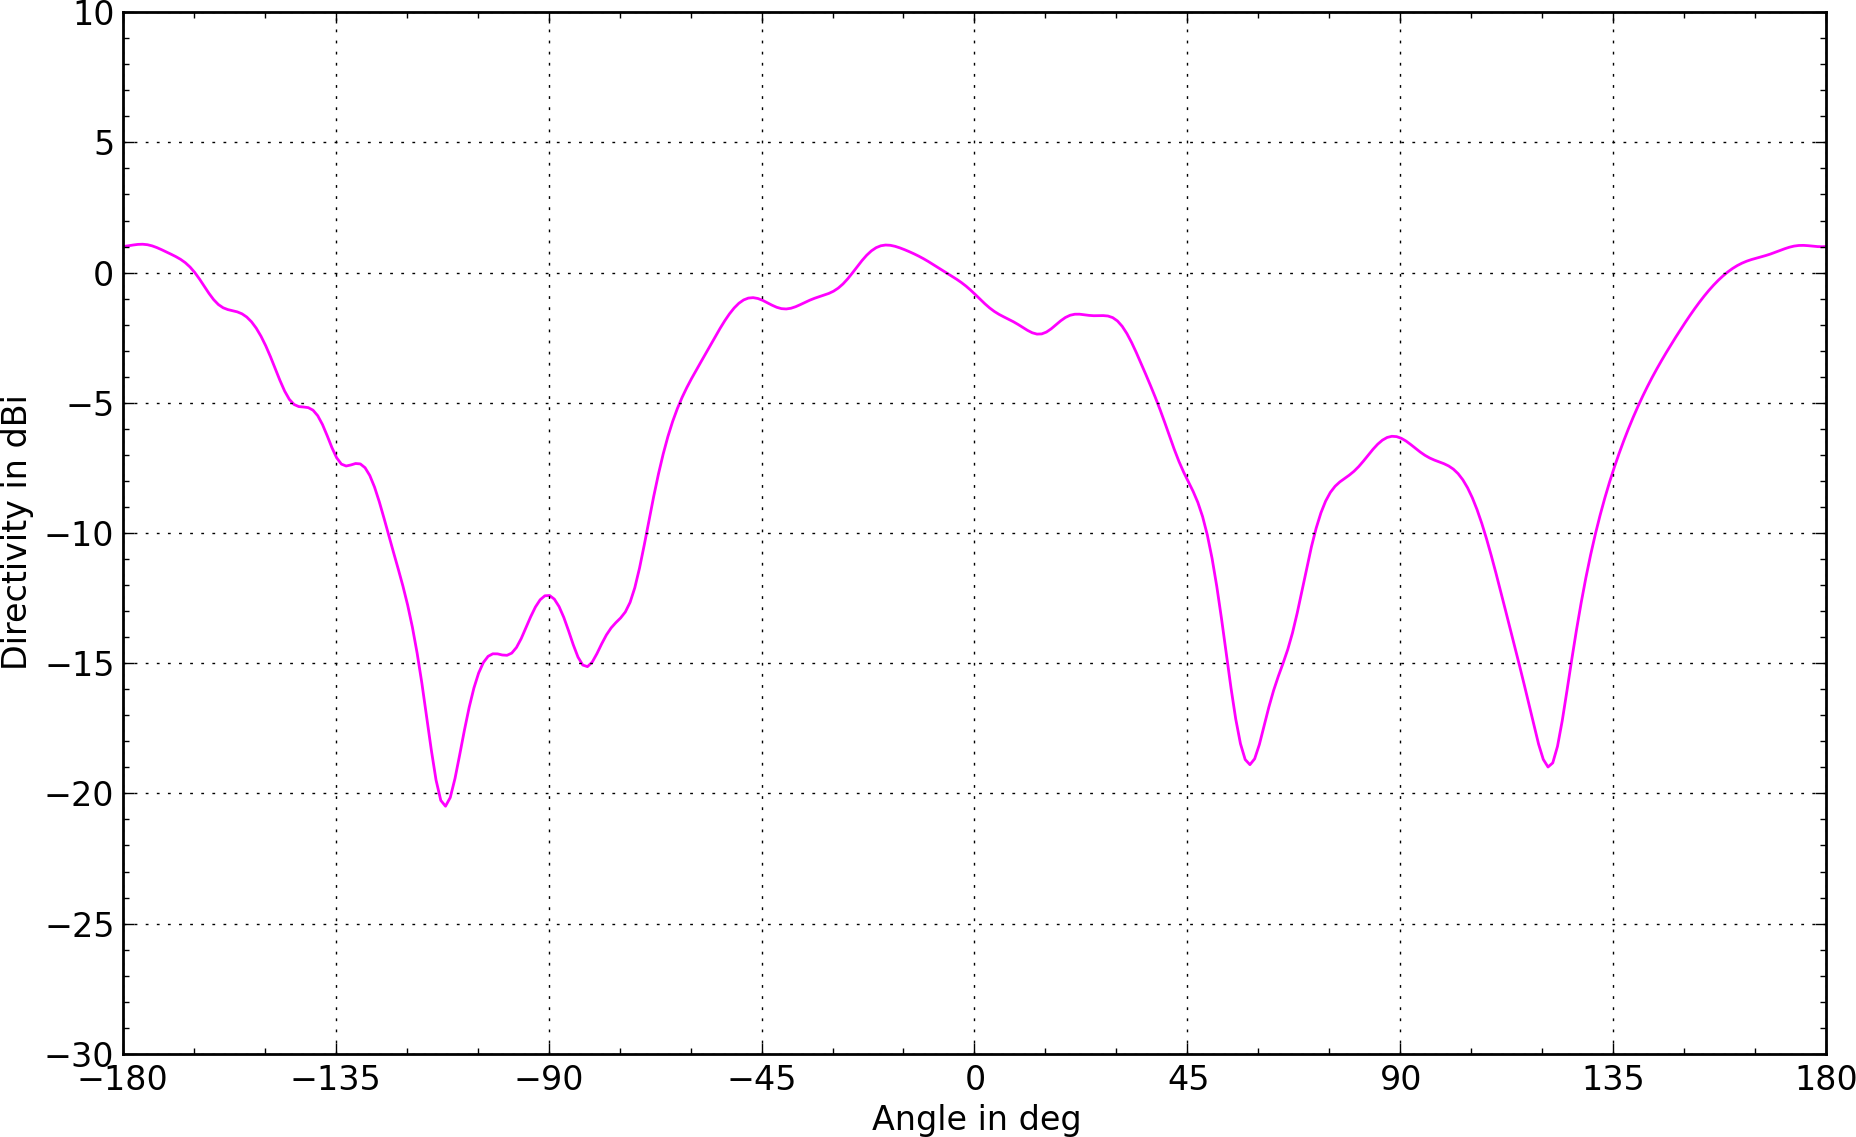
\includegraphics[width=1\textwidth]{../fig/plt/crazy_stuff_l4_pcb_v2c_laptop_1a_105_5ghz0_ephi_phi90-trim.png}
		\caption{$\vec{E_{\varphi}}$ mit $\varphi=\SI{90}{\degree}$ bei \SI{5.0}{\giga\hertz}}
	\end{subfigure}

	\begin{subfigure}[b]{0.48\textwidth}
		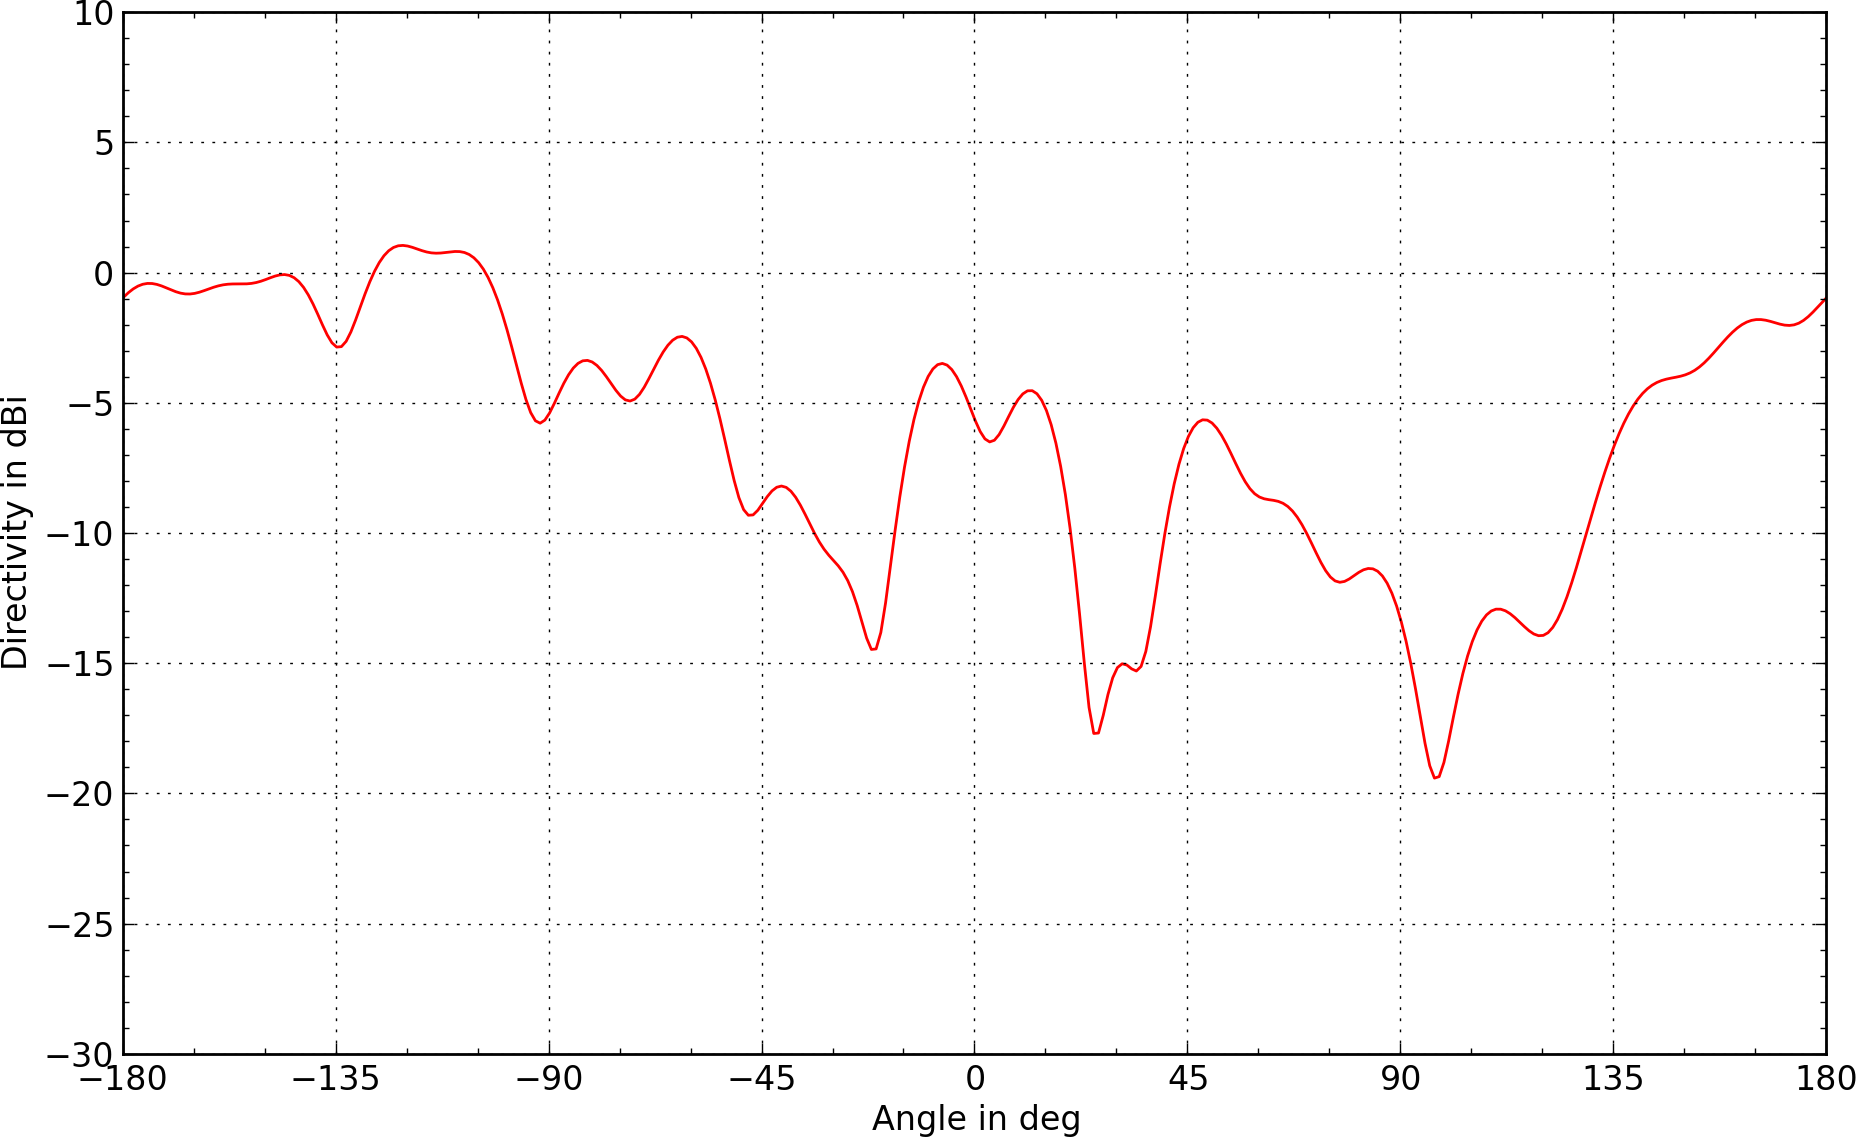
\includegraphics[width=1\textwidth]{../fig/plt/crazy_stuff_l4_pcb_v2c_laptop_1a_105_2ghz4_etheta_phi90-trim.png}
		\caption{$\vec{E_{\theta}}$ mit $\varphi=\SI{90}{\degree}$ bei \SI{2.4}{\giga\hertz}}
	\end{subfigure}
	\begin{subfigure}[b]{0.48\textwidth}
		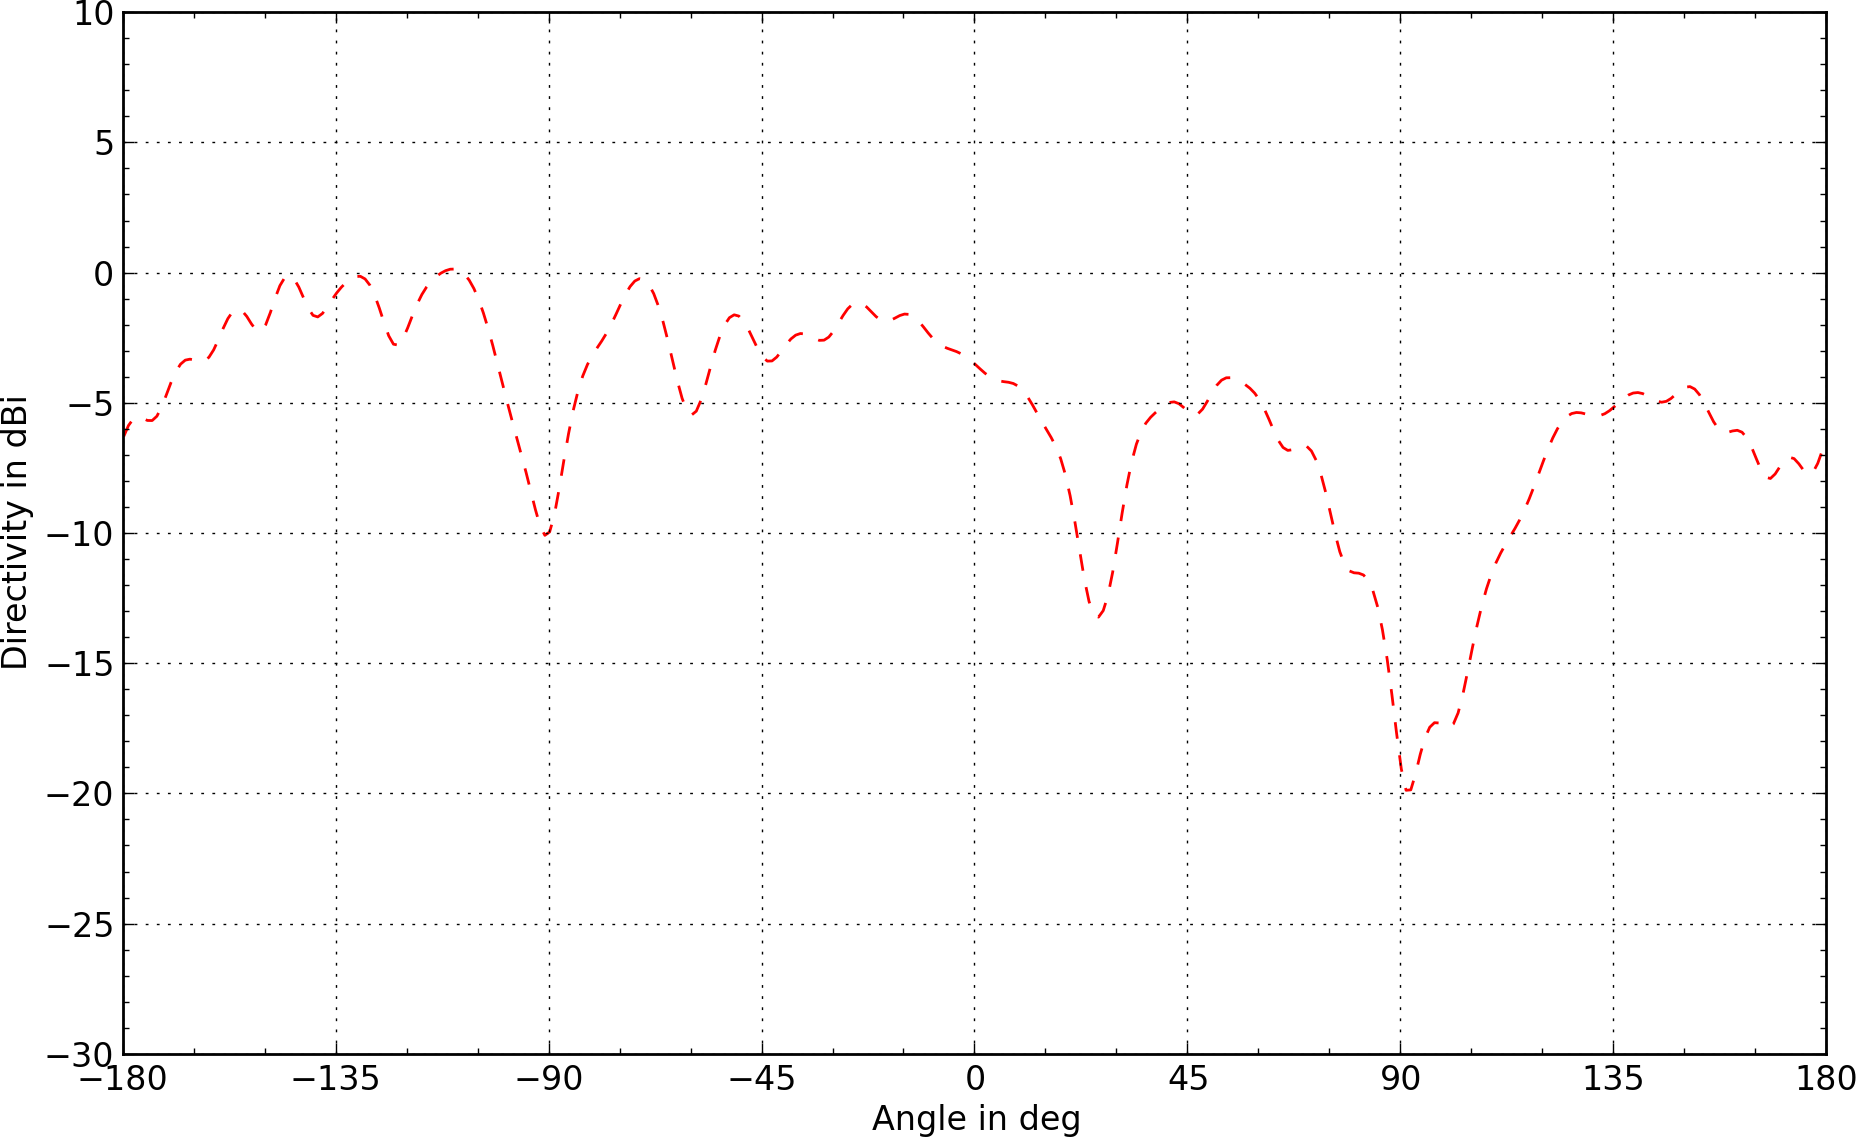
\includegraphics[width=1\textwidth]{../fig/plt/crazy_stuff_l4_pcb_v2c_laptop_1a_105_5ghz0_etheta_phi90-trim.png}
		\caption{$\vec{E_{\theta}}$ mit $\varphi=\SI{90}{\degree}$ bei \SI{5.0}{\giga\hertz}}
	\end{subfigure}
	\caption[1D Simulationen mit Empite für $\vec{E_{tot}}$, $\vec{E_{\varphi}}$ und $\vec{E_{\theta}}$]{
		1D Messungen mit StarLab für $\vec{E_{tot}}$, $\vec{E_{\varphi}}$ und $\vec{E_{\theta}}$.
		Die Abbildung zeigt die gemessenen Verläufe für die
		verschiedenen Vektoren bei fixiertem
		$\varphi = \SI{90}{\degree}$ mit eingestecktem
		Stick im Port 1A des Laptop bei einem Stellwinkel
		des Bildschirms von \SI{105}{\degree}.}
\end{figure}

